\begin{answer}{davidbeckhamparty}
The best way to solve this is to draw an adjacency matrix,
that is, a matrix filled with zeros and ones, where
row $i$ contains a one in column $j$ if person $i$ knows person $j$.
Let $\text{knows}(i,i)=0$, so the matrix has zeros on its diagonal:

\begin{center}
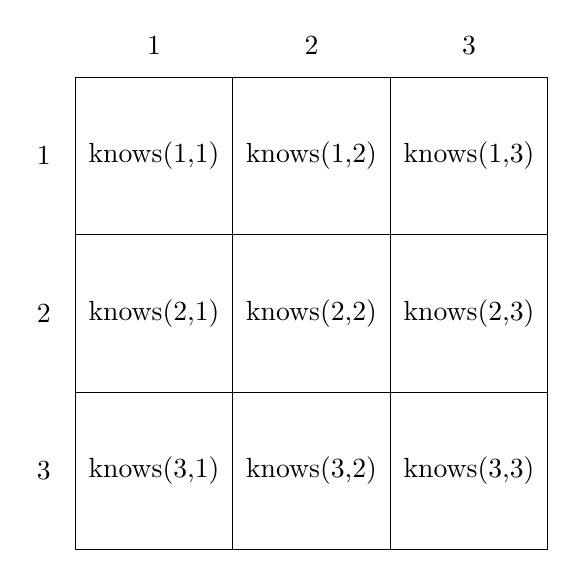
\begin{tikzpicture}[scale=2]
% Draw the numbers outside the matrix
\foreach \i in {1,...,3}
{
\draw (0.3,-\i) node{\i};
\draw (\i,-0.3) node{\i};
}
% Draw the matrix
\foreach \x in {1,...,3}
\foreach \y in {1,...,3}
{
\draw (\x,-\y) +(-.5,-.5) rectangle ++(.5,.5);
\draw (\x,-\y) node (n\y\x) {knows(\y,\x)}; %reverse the x and y to give the expected behaviour
}
\end{tikzpicture}
\end{center}
Think about what this matrix would look like given the conditions of the party in the question.
I draw a $9 \times 9$ matrix here, but you can quickly draw a smaller one to get the gist of it.
The important thing to realise is that David Beckham’s row will be empty, and his columns will be filled with ones (except for the diagonal element):
\begin{center}
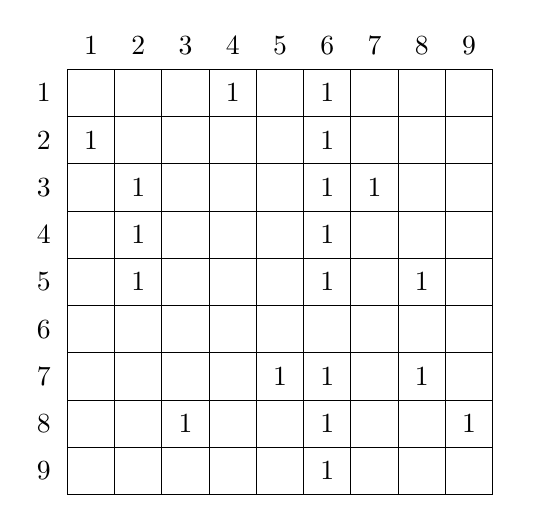
\begin{tikzpicture}[scale=0.6]
% Draw the numbers outside the matrix
\foreach \i in {1,...,9}
{
\draw (0,-\i) node{\i};
\draw (\i,0) node{\i};
}
% Draw the matrix
\foreach \x in {1,...,9}
{
  % Make nodes on the outside of the matrix on the right side
  % Label them with o1, o2, etc.
  \draw (10,-\x) node (o\x) {};
  \foreach \y in {1,...,9}
  {
    \draw (\x,-\y) +(-.5,-.5) rectangle ++(.5,.5);
    % Make the node a circle for space reasons, but don't draw it
    \draw (\x,-\y) node[circle, inner sep=2mm] (n\y\x) {}; %reverse the x and y to give the expected behaviour
  }
}
% Draw some ones
% David Beckham is person 6
% %Everyong knows someone, except Beckham
\draw (n14) node{1};
\draw (n21) node{1};
\draw (n32) node{1} (n37) node{1};
\draw (n42) node{1};
\draw (n52) node{1} (n58) node{1};
% Beckham's row
\draw (n78) node{1} (n75) node{1};
\draw (n83) node{1} (n89) node{1};

%Everyone knows David Beckham
\draw (n16) node{1};
\draw (n26) node{1};
\draw (n36) node{1};
\draw (n46) node{1};
\draw (n56) node{1};
\draw (n76) node{1};
\draw (n86) node{1};
\draw (n96) node{1};
\end{tikzpicture}
\end{center}
You can use the function to fill in values until you find David Beckham,
but filling the whole matrix is expensive. For $n$ people, you would need $n^2$ evaluations of the function.
You need to find a smarter way to find Beckham's row.

Start with person 1 and find the first non-zero entry for their row.
You have now learned two things:
\begin{enumerate}
  \item Person 1 is not David Beckham, because Beckham doesn't know anyone at the party
  \item All the people who person 1 doesn't know can be disregarded: they are not Beckham (everyone at the party knows David Beckham, so if person 1 doesn't know you, you \emph{can't} be David Beckham)
\end{enumerate}
The second point is the crux.
If you don't identify it immediately, talk through the problem and hopefully the interviewer will nudge you in the right direction.
You will use this knowledge to rapidly discount whole blocks of people as ``not Beckham''.
Start at person 1 and check their row.
When you find a one, jump to that person (who might be David Beckham).
Every zero you find discounts its corresponding person as not being Beckham; conversely, when you find a one, you know the current person is also not Beckham.
If you get to the end of any row, that row represents David Beckham.
This method only requires $n$ evaluations of the function since you only need to traverse all the columns, as seen in the diagram below:

\begin{center}
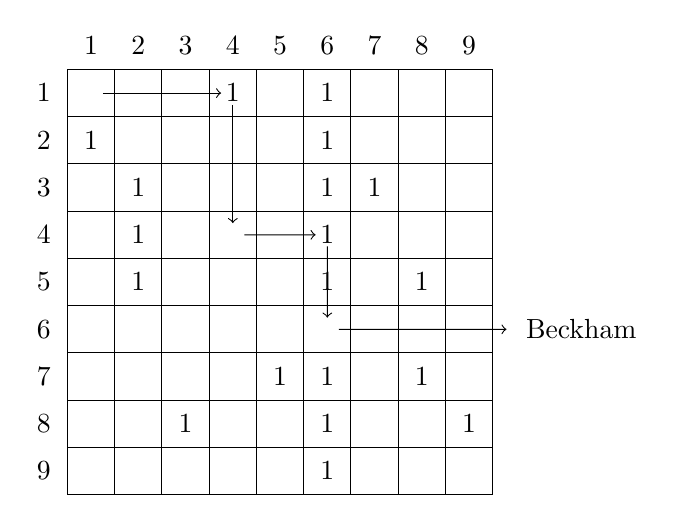
\begin{tikzpicture}[scale=0.6]
% Draw the numbers outside the matrix
\foreach \i in {1,...,9}
{
\draw (0,-\i) node{\i};
\draw (\i,0) node{\i};
}
% Draw the matrix
\foreach \x in {1,...,9}
{
  % Make nodes on the outside of the matrix on the right side
  % Label them with o1, o2, etc.
  \draw (10,-\x) node (o\x) {};
  \foreach \y in {1,...,9}
  {
    \draw (\x,-\y) +(-.5,-.5) rectangle ++(.5,.5);
    % Make the node a circle for space reasons, but don't draw it
    \draw (\x,-\y) node[circle, inner sep=1mm] (n\y\x) {}; %reverse the x and y to give the expected behaviour
  }
}
% Draw some ones
% David Beckham is person 6
% %Everyong knows someone, except Beckham
\draw (n14) node{1};
\draw (n21) node{1};
\draw (n32) node{1} (n37) node{1};
\draw (n42) node{1};
\draw (n52) node{1} (n58) node{1};
% Beckham's row
\draw (n78) node{1} (n75) node{1};
\draw (n83) node{1} (n89) node{1};

%Everyone knows David Beckham
\draw (n16) node{1};
\draw (n26) node{1};
\draw (n36) node{1};
\draw (n46) node{1};
\draw (n56) node{1};
\draw (n76) node{1};
\draw (n86) node{1};
\draw (n96) node{1};

\draw[->] (n11) to (n14);
\draw[->] (n14) to (n44);
\draw[->] (n44) to (n46);
\draw[->] (n46) to (n66);
\draw[->] (n66) to (o6) node[anchor=west]{Beckham};

\end{tikzpicture}
\end{center}

If Victoria Beckham is also at a party with nine people, the matrix might look like the following example, where David and Victoria are individuals 4 and 6:
\begin{center}
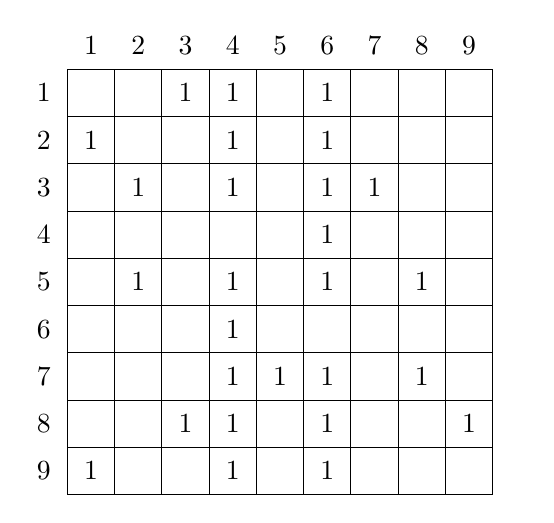
\begin{tikzpicture}[scale=0.6]
% Draw the numbers outside the matrix
\foreach \i in {1,...,9}
{
\draw (0,-\i) node{\i};
\draw (\i,0) node{\i};
}
% Draw the matrix
\foreach \x in {1,...,9}
{
  % Make nodes on the outside of the matrix on the right side
  % Label them with o1, o2, etc.
  \draw (10,-\x) node (o\x) {};
  \foreach \y in {1,...,9}
  {
    \draw (\x,-\y) +(-.5,-.5) rectangle ++(.5,.5);
    % Make the node a circle for space reasons, but don't draw it
    \draw (\x,-\y) node[circle, inner sep=2mm] (n\y\x) {}; %reverse the x and y to give the expected behaviour
  }
}
% Draw some ones
% David Beckham is person 6
% %Everyong knows someone, except Beckham
\draw (n13) node{1};
\draw (n21) node{1};
\draw (n32) node{1} (n37) node{1};
 %Victoria's row
\draw (n52) node{1} (n58) node{1};
 % Beckham's row
\draw (n78) node{1} (n75) node{1};
\draw (n83) node{1} (n89) node{1};
\draw (n91) node{1};


%Everyone knows David Beckham and Victoria
\draw (n14) node{1} (n16) node{1};
\draw (n24) node{1} (n26) node{1};
\draw (n34) node{1} (n36) node{1};
\draw               (n46) node{1};
\draw (n54) node{1} (n56) node{1};
\draw (n64) node{1}              ;
\draw (n74) node{1} (n76) node{1};
\draw (n84) node{1} (n86) node{1};
\draw (n94) node{1} (n96) node{1};

\end{tikzpicture}
\end{center}
The same logic as before applies.
Start at the first person, and ask whether they know person $2, 3, 4, \ldots, n$.
Each individual they don't know can be discounted as \emph{neither} Victoria \emph{nor} David.
The last two people visited using this method are David and Victoria Beckham.
(You can't identify which is which, but nor were you asked to.)
Below, the final diagram shows how to traverse the matrix:
\begin{center}
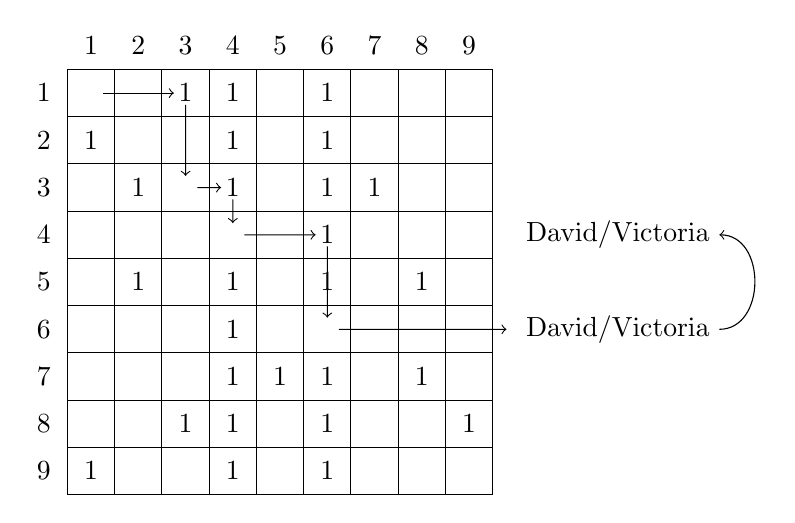
\begin{tikzpicture}[scale=0.6]
% Draw the numbers outside the matrix
\foreach \i in {1,...,9}
{
\draw (0,-\i) node{\i};
\draw (\i,0) node{\i};
}
% Draw the matrix
\foreach \x in {1,...,9}
{
  % Make nodes on the outside of the matrix on the right side
  % Label them with o1, o2, etc.
  \draw (10,-\x) node (o\x) {};
  \foreach \y in {1,...,9}
  {
    \draw (\x,-\y) +(-.5,-.5) rectangle ++(.5,.5);
    % Make the node a circle for space reasons, but don't draw it
    \draw (\x,-\y) node[circle, inner sep=1mm] (n\y\x) {}; %reverse the x and y to give the expected behaviour
  }
}
% Draw some ones
% David Beckham is person 6
% %Everyong knows someone, except Beckham
\draw (n13) node{1};
\draw (n21) node{1};
\draw (n32) node{1} (n37) node{1};
 %Victoria's row
\draw (n52) node{1} (n58) node{1};
 % Beckham's row
\draw (n78) node{1} (n75) node{1};
\draw (n83) node{1} (n89) node{1};
\draw (n91) node{1};


%Everyone knows David Beckham and Victoria
\draw (n14) node{1} (n16) node{1};
\draw (n24) node{1} (n26) node{1};
\draw (n34) node{1} (n36) node{1};
\draw               (n46) node{1};
\draw (n54) node{1} (n56) node{1};
\draw (n64) node{1}              ;
\draw (n74) node{1} (n76) node{1};
\draw (n84) node{1} (n86) node{1};
\draw (n94) node{1} (n96) node{1};

\draw[->] (n11) to (n13);
\draw[->] (n13) to (n33);
\draw[->] (n33) to (n34);
\draw[->] (n34) to (n44);
\draw[->] (n44) to (n46) ;
\draw[->] (n46) to (n66);
\draw[->] (n66) to (o6);
\node (exita) at (o6) [anchor=west] {David/Victoria};
\node (exitb) at (o4) [anchor=west] {David/Victoria};
\draw[->] (exita.east) .. controls ++(1,0) and ++(1,0) .. (exitb.east);

\end{tikzpicture}
\end{center}
This question tests your knowledge of applied graph or network theory, and it has more to do with computer algorithms than mathematics.
\index{graph theory}
While these kinds of questions aren't that prevalent, they are increasingly common at some hedge funds and high-frequency trading firms who emphasise algorithms and programming skills.
If you are required to do a pre-interview coding test, chances are you will see a graph theory problem.
They used to be popular in Google interviews back when they still asked brainteasers.
Google has since stopped doing this after discovering that brainteaser performance was a bad predictor of actual job performance.\footnote{See, for instance, this newspaper article by \citet{GoogleBrainteasers}.}

\end{answer}
